\chapter{Resource Locations}
\label{1}

\abstract{This chapter defines resources and their locations in the file system.}

\section{What is a resource?}
\label{sec:1}
Use the template

\begin{equation}
a \times b = c\;,
\end{equation}


\begin{eqnarray}
a \times b = c \nonumber\\
\vec{a} \cdot \vec{b}=\vec{c}
\label{eq:01}
\end{eqnarray}


%puts image at the bottom of the page
\begin{figure}[b]
\sidecaption
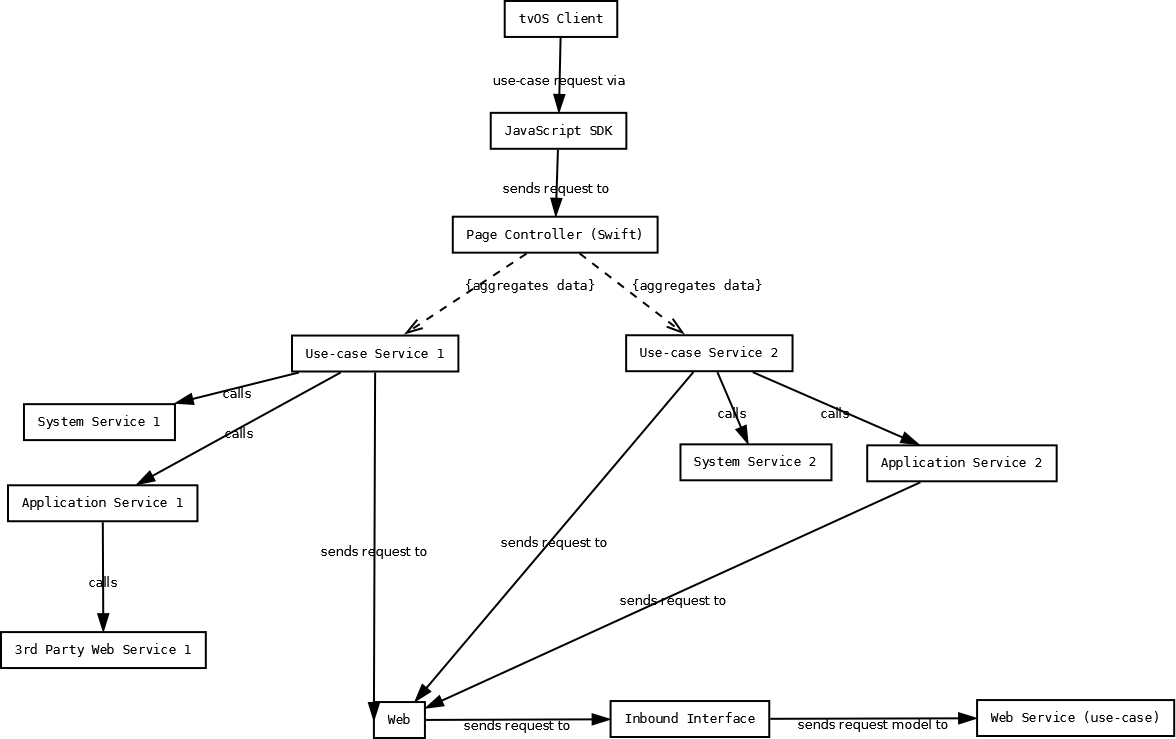
\includegraphics[scale=.20]{figure.png}
\caption{If the width of the}
\label{fig:1}
\end{figure}


\paragraph{Paragraph Heading}
Instead of simply


%puts image at the top of the page
\begin{figure}[t]
\sidecaption[t]
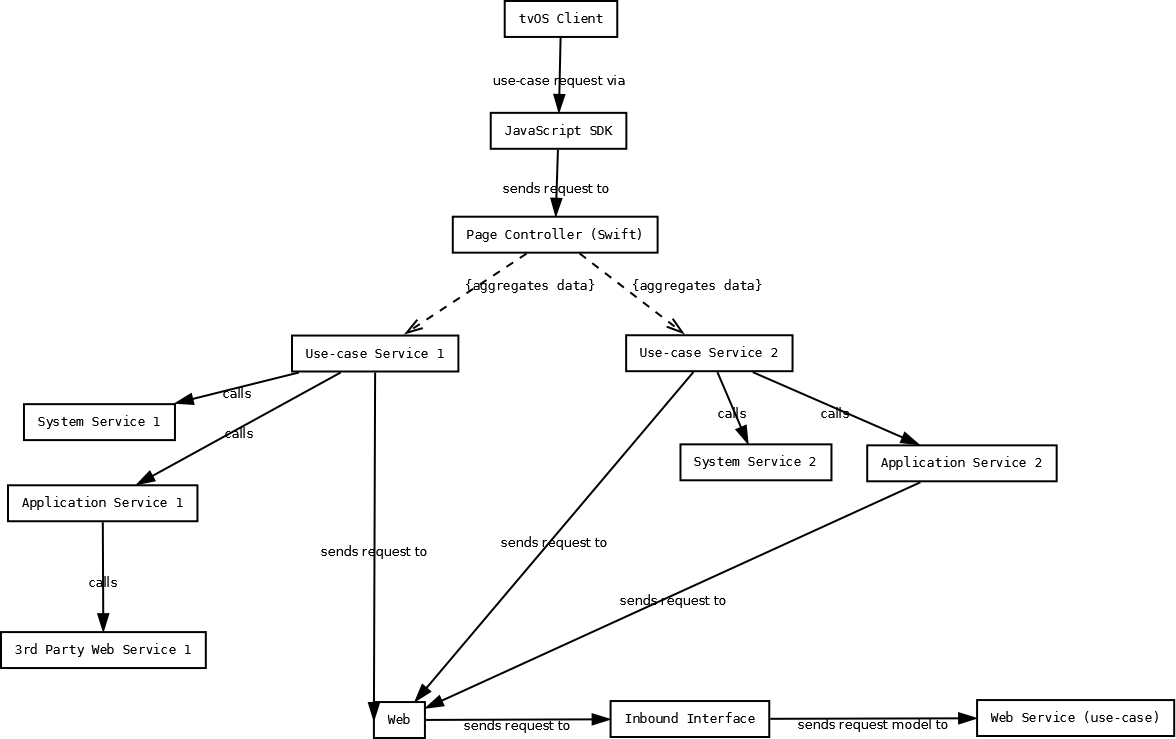
\includegraphics[scale=.20]{figure.png}
\caption{Please write your figure caption here}
\label{fig:2}       % Give a unique label
\end{figure}

\runinhead{Run-in Heading Boldface Version} Use the \LaTeX\ automatism for all your cross-references and citations as has already been described in Sect.~\ref{sec:2}.

\begin{table}
\caption{Please write your table caption here}
\label{tab:1}
    \begin{tabular}{p{2cm}p{2.4cm}p{2cm}p{4.9cm}}
    \hline\noalign{\smallskip}
    Classes & Subclass & Length & Action Mechanism  \\
    \noalign{\smallskip}\svhline\noalign{\smallskip}
    Translation & mRNA$^a$  & 22 (19--25) & Translation repression, mRNA cleavage\\
    Translation & mRNA cleavage & 21 & mRNA cleavage\\
    Translation & mRNA  & 21--22 & mRNA cleavage\\
    Translation & mRNA  & 24--26 & Histone and DNA Modification\\
    \noalign{\smallskip}\hline\noalign{\smallskip}
    \end{tabular}
$^a$ Table foot note (with superscript)
\end{table}

\begin{description}[Type 1]
\item[Type 1]{That addresses central themes pertainng to migration, health, and disease. In Sect.~\ref{sec:1}, Wilson discusses the role of human migration in infectious disease distributions and patterns.}
\item[Type 2]{That addresses central themes pertainng to migration, health, and disease. In Sect.~\ref{subsec:2}, Wilson discusses the role of human migration in infectious disease distributions and patterns.}
\end{description}

\begin{theorem}
Theorem text goes here.
\end{theorem}

\begin{definition}
Definition text goes here.
\end{definition}

\begin{proof}
Proof text goes here.
\qed
\end{proof}